\documentclass[12pt,oneside,a4paper]{article} % for sharing
\usepackage{apacite}
\usepackage{appendix}
\usepackage{amsmath}
\usepackage{amsthm}

\usepackage{amssymb} % for approx greater than
\usepackage{caption}
\usepackage{placeins} % for \FloatBarrier
\usepackage{graphicx}
\usepackage{subcaption}
\usepackage{longtable}
\usepackage{setspace}
\usepackage{booktabs}
\usepackage{tabularx}
\usepackage{xcolor,colortbl}
\usepackage{chngpage}
\usepackage{natbib}
\bibpunct{(}{)}{,}{a}{}{;} 
\usepackage{url}
\usepackage{nth}
\usepackage{authblk}
\usepackage[most]{tcolorbox}
\usepackage[normalem]{ulem}
\usepackage{amsfonts}
% columns for longtable
\usepackage{arydshln} % Dashed lines in matrices

\usepackage[margin=1in]{geometry}
%\doublespacing % for review

% line numbers to make review easier
%\usepackage{lineno}
%\linenumbers

%\usepackage{soul}% for \st{}

%%%%%%%%%%%%%%%%%%%%%%%%%%%%%%%%%%%%%%%%%%%%%%%%%%%%%%%%%%%%%%%%%%%%%%%%%%%%%%
% for section 4 math environments
\theoremstyle{definition}
\newtheorem{definition}{Definition}[section]
\newtheorem{theorem}{Theorem}[section]
\newtheorem{proposition}{Proposition}[section]
\newtheorem{corollary}{Corollary}[proposition]
\newtheorem{remark}{Remark}[section]

%%%%%%%%%%%%%%%%%%%%%%%%%%%%%%%%%%%%%%%%%%%%%%%%%%%%%%%%%%%%%%%%%%%%%%%%%%%%%%

\newcommand\ackn[1]{%
  \begingroup
  \renewcommand\thefootnote{}\footnote{#1}%
  \addtocounter{footnote}{-1}%
  \endgroup
}

% Affiliations in small font size
\renewcommand\Affilfont{\small}

\defcitealias{HMD}{HMD 2016}

% junk for longtable caption
\AtBeginEnvironment{longtable}{\linespread{1}\selectfont}
\setlength{\LTcapwidth}{\linewidth}

% sort van Raalte properly
% #1: sorting key, #2: prefix for citation, #3: prefix for bibliography
\DeclareRobustCommand{\VAN}[3]{#2} % set up for citation
\newcommand{\tc}{\quad\quad\text{,}}
\newcommand{\tp}{\quad\quad\text{.}}
%%%%%%%%%%%%%%%%%%%%%%%%%%%%%%%
\begin{document}

\title{A note on the stochasticity of population stocks}
%\author{author(s) redacted}
\author[1]{Andrew Noymer\thanks{noymer@uci.edu}}
\author[2]{Tim Riffe}

\affil[1]{University of California, Irvine}
\affil[2]{Max Planck Institute for Demographic Research, Rostock, Germany}



\maketitle

\begin{abstract}
sooo abstract.
\end{abstract}

\section{Background}
The casual observer may be tempted to judge whether or not a population is
longevous by looking at its age pyramid, perhaps taking the proportion of
the population that are centenarians as a measure of how long-lived a population
is. Demographers know better than to trust population stocks for such things,
having established since the 18th Century \citep{graunt1939natural} the
lifetable--- purged of the capricious movements of population stocks--- as the primary instrument to assess
longevity. It is our aim to point out that even under the most ideal of
hypothetical circumstances ---a population closed to migration, renewing with
identically-sized birth cohorts and unchanging mortality rates--- the proportion
of centenarians is so highly variable that is must be understood as unreliable
for the purpousness of measuring the propensity of a population to be
long-lived.

\section{Methods}

We simulate stuff.

\section{Results}

\begin{figure}
\centering
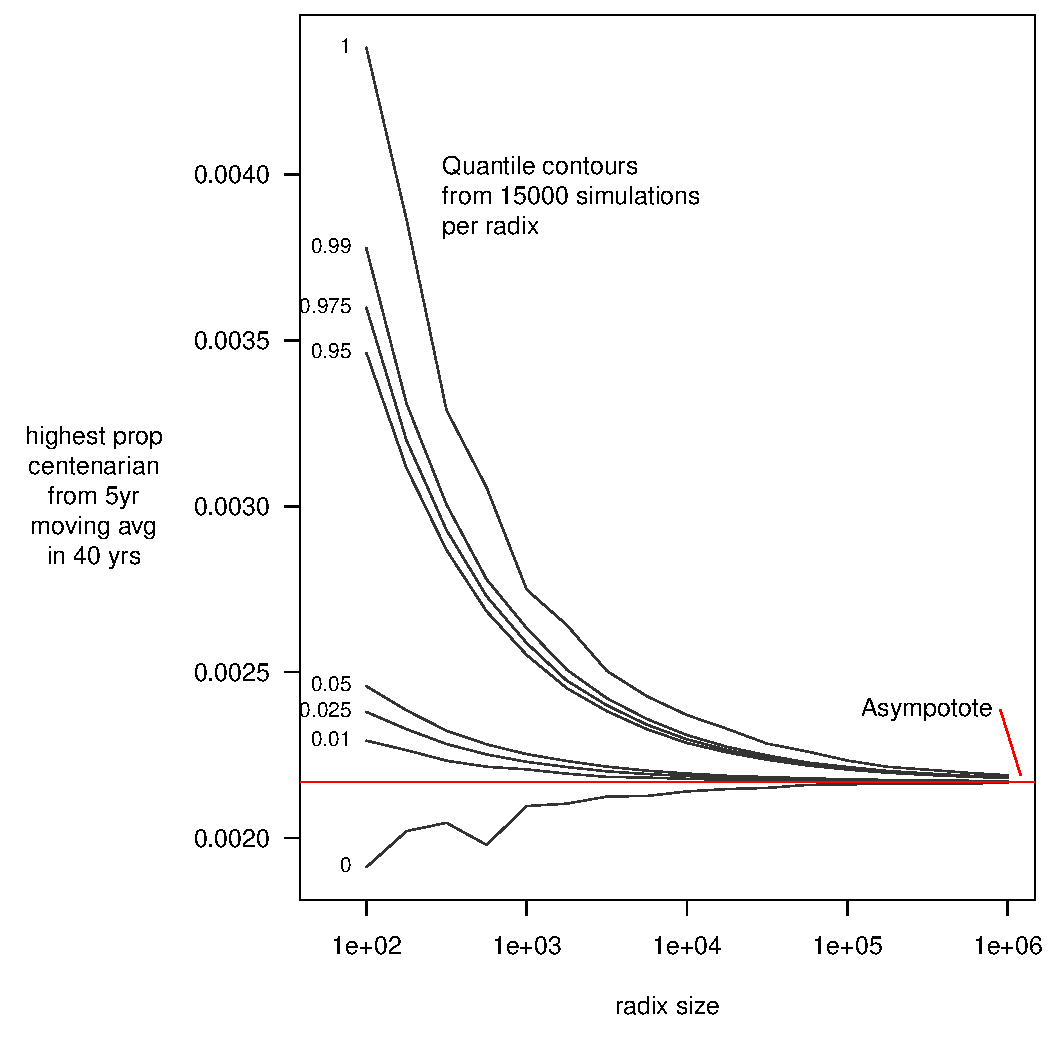
\includegraphics[scale = .8]{Figures/SimJPNf2010.pdf}
\caption{Quantiles High water centenarian proportion}
\end{figure}

\section{Lesson}
Stick to the lifetable folks.

\bibliographystyle{apacite} 
%\bibliographystyle{plainnat}
\bibliography{references.bib} 


\end{document}
